% Chapter 2

\chapter{Analysis} % Main chapter title
\label{chap:Chapter2} % For referencing the chapter elsewhere, use \ref{chap:Chapter3} 

In this chapter it will be presented a bussiness value analysis of the project and the reasoning behind it. 

\section{Engineering requirements}

\dots

\section{Value Analysis}

\dots

\subsection{New concept development model}

\dots

\subsection{Value}

Value for customer, Perceived Value, Benefits, Sacrifices

\dots

\subsection{Value Proposition}

A value proposition is 

\subsection{CANVAS model}

\dots

\begin{figure}[H]
\centering
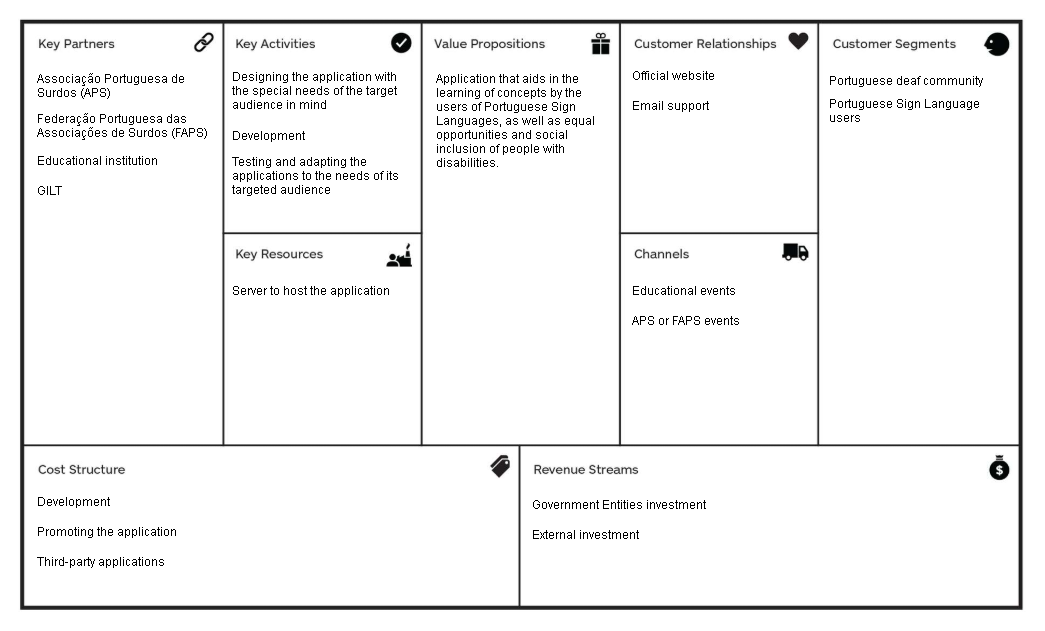
\includegraphics[width=\textwidth,keepaspectratio]{ch2/assets/CANVAS.png}
\caption[CANVAS]{CANVAS model}
\label{fig:CANVAS}
\end{figure}

\subsection{AHP}

\dots

\begin{figure}[H]
\centering
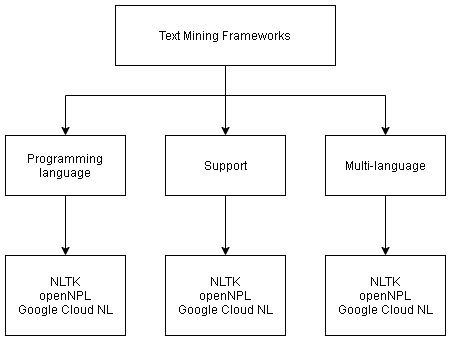
\includegraphics[width=\textwidth,keepaspectratio]{ch2/assets/AHP.png}
\caption[AHP Hierarchy Division]{AHP Hierarchy Division}
\label{fig:AHP}
\end{figure}

As observed in the Figure~\ref{fig:AHP}, the items of the first layer, corresponding to the primary objectives, had the following criteria behind their selection:

\begin{itemize}
    \item Language - Utilize a simple and clear language throughout the website.
    \item Text Transcripts - Provide text transcripts for audio or video content that might be present.
    \item Contact options - In order to better help, and promoting inclusion, provide a diverse and easily accessible contant information page.
    \item Visual balance - Implement a good balance between text and image as well as an easy to use navegation flow.
\end{itemize}


